\RequirePackage{plautopatch}
\documentclass[dvipdfmx,uplatex,report]{jsbook} % \documentclass[a4paper]{jsreport}
\RequirePackage[l2tabu, orthodox]{nag} % 古いコマンド, パッケージに対する警告
\usepackage{amsmath, amssymb, amsfonts, amsthm}
\usepackage{ascmac}
\usepackage{bbm}
\usepackage{bigdelim}
\usepackage{cases}
\usepackage[usenames]{color}
\usepackage{color}
\usepackage{comment}
\usepackage{currfile}
\usepackage{empheq}
\usepackage{fancybox}
\usepackage{graphicx}
\usepackage{here}
\usepackage[dvipdfmx,colorlinks,linkcolor=Blue,urlcolor=blue,bookmarksopenlevel=4]{hyperref}
\usepackage{ifthen}
\usepackage{mathtools}
\usepackage{multirow}
\usepackage{siunitx}
\usepackage{tabularx, arydshln}
\usepackage{udline}
\usepackage{url}

\theoremstyle{definition} % 定理環境:斜体なし
\newtheorem*{commentary}{解説}
\newtheorem*{attention}{注意}
\newtheorem*{solution}{解法}
\newtheorem*{definition}{定義}
\makeatletter
\newcounter{subsubsubsection}
\setcounter{subsubsubsection}{0}
\newcommand{\subsubsubsection}{
	\refstepcounter{subsubsubsection}
	\@startsection{paragraph}{4}{\z@}%
	{1.0\Cvs \@plus.5\Cdp \@minus.2\Cdp}%
	{.1\Cvs \@plus.3\Cdp}%
	{\reset@font\sffamily\normalsize}
}
\makeatother
\setcounter{secnumdepth}{4}

% section, subsection, subsubsection の先頭に部番号が付くようにする
\makeatletter
\@addtoreset{chapter}{part}\renewcommand{\thechapter}{\thepart.\arabic{chapter}}
\@addtoreset{section}{chapter}\renewcommand{\thesection}{\thechapter.\arabic{section}}
\@addtoreset{subsection}{section}\renewcommand{\thesubsection}{\thesection.\arabic{subsection}}
\@addtoreset{subsubsection}{subsection}\renewcommand{\thesubsubsection}{\thesubsection.\arabic{subsubsection}}
\@addtoreset{subsubsubsection}{subsubsection}\renewcommand{\thesubsubsubsection}{\thesubsubsection.\arabic{subsubsubsection}}

\renewcommand{\theequation}{\arabic{equation}} % jsbook によって書き換えられた \theequation を元に戻す

% part, chapter, section, subsection, subsubsection, subsubsubsection 毎に数式,図番号をリセットする
\@addtoreset{equation}{part}
\@addtoreset{equation}{chapter}
\@addtoreset{equation}{section}
\@addtoreset{equation}{subsection}
\@addtoreset{equation}{subsubsection}
\@addtoreset{equation}{subsubsubsection}

\@addtoreset{figure}{part}
\@addtoreset{figure}{chapter}
\@addtoreset{figure}{section}
\@addtoreset{figure}{subsection}
\@addtoreset{figure}{subsubsection}
\@addtoreset{figure}{subsubsubsection}

% @dottedtocline の空白版
\newcommand{\@motchyTocline}[5]{%
	\ifnum #1>\c@tocdepth \else
	\vskip \z@ \@plus.2\p@
	{%
		\leftskip #2\relax \rightskip \@tocrmarg \parfillskip -\rightskip
		\parindent #2\relax\@afterindenttrue
		\interlinepenalty\@M
		\leavevmode
		\@lnumwidth #3\relax
		\advance\leftskip \@lnumwidth \null\nobreak\hskip -\leftskip
		\textbf{\footnotesize #4}\nobreak
		\leaders\hbox{$\m@th \mkern \@dotsep mu\hbox{\quad}\mkern \@dotsep
		mu$}\hfill \nobreak\hb@xt@\@pnumwidth{%
		\hfil\normalfont \normalcolor #5}\par%
	}\fi%
}

% 目次の番号とタイトルが重ならないようにする
% dottedtocline{A}{B}{C}のパラメータABC
%   A:目次を生成するレベル(\chapterはレベル0、\sectionはレベル1...)
%   B:一番外側からの左マージン
%   C:見出し番号が入るボックスの幅
\renewcommand{\l@chapter}{\@motchyTocline{0}{0em}{7em}}
\renewcommand{\l@section}{\@dottedtocline{1}{1em}{7em}}
\renewcommand{\l@subsection}{\@dottedtocline{2}{2em}{6em}}
\renewcommand{\l@subsubsection}{\@dottedtocline{3}{3em}{5em}}
\makeatother

\setcounter{tocdepth}{4} % subsubsubsection まで目次に表示する

\input{macros/LaTeX-motchyMacros/motchyMacros}

\begin{document}
	\title{motchyの信号処理備忘録}
	\author{motchy}
	\date{\西暦 2019年11月16日 $\sim$ \today \\ver 0.3.0}
	\maketitle
	{\scriptsize \tableofcontents}

	\newcommand{\cycConv}[2]{\underset{\text{cyc}}{{#1}*{#2}}}

	 \part{表記法}
		\chapter{数学記号}
			\begin{itemize}
				\item $\field$: 体
				\item $\integers$: 整数全体の集合
				\item $\realSpace$: 実数全体の集合
				\item $\complexSpace$: 複素数全体の集合
				\item $\bm{a}/\bm{b}\;(d \in \naturalNumbers,\;\bm{a},\bm{b} \in \field^d,\;b_i\neq 0 \text{ for all }i)$: $[a_1/b_1,\cdots,a_d/b_d]^\top$
				\item $a\%b\;(a,b\in\integers,\;b\neq 0)$: $a$を$b$で割った余り。符号に2通り考えられるが、本書では結果を0以上$|a|$未満とする定義を採用する。
				\item $\bm{a}\%\bm{b}\;(d\in\naturalNumbers,\;\bm{a},\bm{b} \in \integers^d,\; b_i\neq 0 \text{ for all }i)$: $[a_1\%b_1,\cdots,a_d\%b_d]^\top$
			\end{itemize}
		
		\chapter{連続座標信号の表現}
			連続的な座標値$\bm{x}\in\realSpace^{d_1}\;(d_1\in\naturalNumbers)$から$\realSpace^{d_2}\;(d_2\in\naturalNumbers)$への写像を$d_1$次元連続座標信号という。
			信号値は全ての座標に対して定義される必要はない。
			\par
			例えばカセットテープレコーダーに記録された音声信号は$d_1=d_2=1$のものである。
			\par
			信号$f$の位置$\bm{x} = [x_1,x_2,\cdots,x_{d_1}]^\top$での値を$f(\bm{x})$や$f(x_1,\cdots,x_{d_1})$で表す。

		\chapter{離散座標信号の表現}
			離散的な座標値$\bm{x}\in\integers^{d_1}\;(d_1\in\naturalNumbers)$から$\realSpace^{d_2}\;(d_2\in\naturalNumbers)$への写像を$d_1$次元離散座標信号という。
			信号値は全ての座標に対して定義される必要はない。
			\par
			例えば離散的な時刻での電圧のサンプリングデータは$d_1=d_2=1$のものである(この場合の「座標」は時間軸上での座標という意味になる)。
			また、コンピュータのディスプレイに映る2次元カラー画像は$d_1=2,d_2=3$のものである。
			\par
			信号$f$の位置$\bm{x} = [x_1,x_2,\cdots,x_{d_1}]^\top$での値を$f(\bm{x})$や$f(x_1,\cdots,x_{d_1})$で表す。

	\part{畳み込み}
	\chapter{畳み込みの微分}
		\section{関係式}
			\begin{shadebox}
				微分可能な複素数値信号 $x_1, x_2:\realNumbers\to\complexNumbers$ に畳み込みが存在するとき、次が成り立つ。
				\[ \derivLong{(x_1*x_2)(t)}{t}{} = {x_1}'*x_2 = x_1*{x_2}' \]
			\end{shadebox}
			\begin{proof}
				\quad\par
				まず次式が成り立つ。
				\begin{align*}
					\derivLong{(x_1*x_2)(t)}{t}{} &= \derivLong{\integrate{-\infty}{\infty}{x_1(\tau)x_2(t-\tau)}{}{\tau}}{t}{} = \integrate{-\infty}{\infty}{x_1(\tau)\derivLong{x_2(t-\tau)}{t}{}}{}{\tau} \\
					&= \integrate{-\infty}{\infty}{x_1(\tau){x_2}'(t-\tau)}{}{\tau} = (x_1*{x_2}')(t)
				\end{align*}
				$x_1*x_2 = x_2*x_1$ を用いて上記と同様の計算を行うと次式が成り立つ。
				\[ \derivLong{(x_1*x_2)(t)}{t}{} = ({x_1}'*x_2)(t) \]
			\end{proof}
		\section{使いどころ}
			例えばディジタル信号処理で役立つときがある。
			前記の関係式の離散座標版も同様に成り立つ。
			(a) 長い入力信号に(b) (それに比べて短い)時間的に変化しない信号(典型的には FIR フィルタの係数)を畳み込むとき、後者の時間微分(典型的には差分で近似)を予め計算しておいて (a) と畳み込めば、微分のオンライン計算が不要になる。
	\chapter{巡回畳み込み}
		\label{巡回畳み込み}
		$\Omega \coloneqq \{0,1,\dots,N_1-1\}\times\{0,1,\dots,N_2-1\}\times\cdots\times\{0,1,\dots,N_d-1\}$とする。
		$f,g$を周期が$(N_1,\dots,N_d)$であるような離散座標信号$f,g: \Omega\to\complexNumbers;\;\bm{n} = [n_1,n_2,\dots,n_d]^\top \mapsto f(\bm{n}),g(\bm{n})$とする。
		$\bm{N} \coloneqq [N_1,\dots,N_d]^\top$とする。
		$f$と$g$の巡回畳み込み$\cycConv{f}{g}$を次式で定義する。
		\[ \left(\cycConv{f}{g}\right)(\bm{n}) \coloneqq \sum_{\bm{m} \in\Omega} f(\bm{m})g((\bm{n}-\bm{m})\%\bm{N}) \]

		\section{巡回畳み込みの可換則}
			\begin{shadebox}
				$\Omega,f,g$の定義を\ref{巡回畳み込み}と同じものとするとき、次が成り立つ。
				\[ \cycConv{f}{g} = \cycConv{g}{f} \]
			\end{shadebox}
			\begin{proof}
				\begin{align}
					\left(\cycConv{g}{f}\right)(\bm{n}) &= \sum_{\bm{m}\in\Omega} g(\bm{m})f((\bm{n}-\bm{m})\%\bm{N}) \nonumber \\
					&= \sum_{m_1=0}^{N_1-1}\sum_{\bm{m}_2\in\Omega_2}g(m_1,\bm{m}_2)f((n_1 - m_1)\%N_1,(\bm{n_2}-\bm{m_2})\%\bm{N_2})
				\end{align}
				ここに$\bm{n}_i \coloneqq [n_i,\dots,n_d]^\top\;(\bm{m}_i,\bm{N}_i\text{も同様}),\;\Omega_i \coloneqq \{0,1,\dots,N_i-1\}\times\cdots\times\{0,1,\dots,N_d-1\}$である。
				\begin{align*}
					(1) &= \sum_{m_1=0}^{n_1}\sum_{\bm{m}_2\in\Omega_2}g(m_1,\bm{m}_2)f(n_1 - m_1,(\bm{n_2}-\bm{m_2})\%\bm{N_2}) \\
					&\quad + \sum_{m_1=n_1+1}^{N_1-1}\sum_{\bm{m}_2\in\Omega_2}g(m_1,\bm{m}_2)f(n_1 + N_1 - m_1,(\bm{n_2}-\bm{m_2})\%\bm{N_2}) \\
					&= \sum_{l_1=n_1}^0 \sum_{\bm{m}_2\in\Omega_2}g(n_1 - l_1,\bm{m}_2)f(l_1,(\bm{n_2}-\bm{m_2})\%\bm{N_2}) \\
					&\quad + \sum_{l_1=N_1-1}^{n_1+1}\sum_{\bm{m}_2\in\Omega_2}g(n_1+N_1-l_1,\bm{m}_2)f(l_1,(\bm{n_2}-\bm{m_2})\%\bm{N_2}) \\
					&= \sum_{l_1=n_1}^0 \sum_{\bm{m}_2\in\Omega_2}g(\textcolor{darkpastelgreen}{(n_1-l_1)\%N_1},\bm{m}_2)f(l_1,(\bm{n_2}-\bm{m_2})\%\bm{N_2}) \\
					&\quad + \sum_{l_1=N_1-1}^{n_1+1}\sum_{\bm{m}_2\in\Omega_2}g((n_1-l_1)\%N_1,\bm{m}_2)f(l_1,(\bm{n_2}-\bm{m_2})\%\bm{N_2}) \\
					&= \sum_{l_1=0}^{N_1-1} \sum_{\bm{m}_2\in\Omega_2}g((n_1-l_1)\%N_1,\bm{m}_2)f(l_1,(\bm{n_2}-\bm{m_2})\%\bm{N_2}) \\
				\end{align*}
				同様の変形を繰り返すと最終的に次のようになる。
				\[ \left(\cycConv{g}{f}\right)(\bm{n}) = \sum_{\bm{l}\in\Omega} g((\bm{n}-\bm{l})\%\bm{N})f(\bm{l}) = \left(\cycConv{f}{g}\right)(\bm{n}) \]
			\end{proof}
		\chapter{諸定理}
			\section{線形変換と畳み込みの順序交換}
				\subsection{動機}
					画像処理に於いてカーネルとの畳み込みを実行してから線形変換を施す場合と、事前に画像とカーネルの両方に線形変換を施してから畳み込む場合の結果の違いに関心がある。
				\subsection{理論}
					$d\in\naturalNumbers$とし、$f:\bm{x}\in\realNumbers^d\mapsto f(\bm{x})\in\realNumbers$を$d$次元信号とする。
					線形変換を表す正則行列を$A$とし、$A$による変換を$T_A$と表す。
					$T_A$による変換は次式を以て定義する。
					\[ T_A(f)(\bm{x}) = f(A^{-1}\bm{x}) \]
					$G:\bm{x}\in\realNumbers^d\mapsto G(\bm{x})\in\realNumbers$を$d$次元信号とする。
					このとき次式が成り立つ。
					\[ T_A(G)*T_A(f) = |A|T_A(G*f) \]
					\begin{proof}
						\quad\par
						$\mu$をJordan測度とする。
						\begin{align*}
							T_A(G)*T_A(f)(\bm{x}) &= \LebInteg{\realNumbers^d}{T_A(G)(\bm{x}-\bm{u})T_A(f)(\bm{u})}{\mu}{\bm{u}} = \LebInteg{\realNumbers^d}{G(A^{-1}(\bm{x}-\bm{u}))f(A^{-1}\bm{u})}{\mu}{\bm{u}} \\
							&= \LebInteg{\realNumbers^d}{G(A^{-1}\bm{x} - A^{-1}\bm{u})f(A^{-1}\bm{u})}{\mu}{\bm{u}} \\
							&= \LebInteg{\realNumbers^d}{G(A^{-1}\bm{x} - \bm{v})f(\bm{v})}{\abs{|A|}\mu}{\bm{v}} \\
							&\phantom{=} (\bm{v}=A^{-1}\bm{u}\text{と変数変換した。}\abs{|A|}\text{は}|A|の絶対値である。) \\
							&= \abs{|A|} \LebInteg{\realNumbers^d}{G(A^{-1}\bm{x} - \bm{v})f(\bm{v})}{\mu}{\bm{v}} \\
							&= \abs{|A|}T_A(G*f)(\bm{x})
						\end{align*}
					\end{proof}
				\section{数値実験}
					Mathematicaによる例が「線形変換と畳み込み.nb」にある。
	 \part{Fourier解析}
		\chapter{Fourier級数展開}
			\section{基底関数}
				Fourier級数展開の基底関数はFourier変換やDFTのものと違って正規化されていないため、美しさに欠ける。
				\par
				$d\in\naturalNumbers,\;W_l>0\;(l=1,2,,\cdots,d),\;\bm{k}\in\integers^d$とする。
				次式で定義される、$\bm{x}\in\realNumbers^d$に関する連続座標信号を、区間$\prod_{l=1}^d [-W_l,W_l]$に於ける第$\bm{k}$基底関数という。
				\[ W(\bm{k},\bm{x}) := \exp i\sum_{l=1}^d k_l\frac{x_l}{W_l}\pi \]

			\section{Fourier係数}
				$d\in\naturalNumbers,\;W_l>0\;(l=1,2,,\cdots,d),\;\Omega:=\prod_{l=1}^d [-W_l,W_l],\;\bm{k}\in\integers^d$とする。
				$f:\bm{x}\in\realNumbers \mapsto f(\bm{x})\in\realNumbers$を、第$l$座標に関して周期が$2W_l$であるような周期関数とする。
				次式で定義する、$\bm{k}$に関する離散座標信号を$f$の第$\bm{k}$Fourier係数という。
				\[ c(f,\bm{k}) := \left(\prod_{l=1}^d 2W_l\right)^{-1}\integ{\Omega}{}{\overline{W(\bm{k},\bm{x})}f(\bm{x})}{\bm{x}} \]

		\chapter{Fourier変換}
			\section{基底関数}
				$d\in\naturalNumbers,\;\bm{x},\bm{\omega}\in\realNumbers^d$とする。
				次のものを$d$次元Fourier変換に於ける基底関数という。
				\[ W(\bm{\omega},\bm{x}) := (2\pi)^{-d/2}\exp i\bm{\omega}^\top\bm{x} \]

			\section{Fourier変換の定義}
				$d\in\naturalNumbers,\;\bm{\omega}\in\realNumbers^d$とする。
				$f:\realNumbers^d\to\complexNumbers$に対して、次式で定義される、$\omega$に関する連続座標信号を$f$のFourier変換という。
				\[ \mathcal{F}(f,\bm{\omega}) := \integ{\realNumbers^d}{}{\overline{W(\bm{\omega},\bm{x})}f(\bm{x})}{\bm{x}} = (2\pi)^{-d/2} \integ{\realNumbers^d}{}{\exp (-i\bm{\omega}^\top\bm{x})f(\bm{x})}{\bm{x}} \]

		\chapter{離散Fourier変換(DFT)}
			\section{基底}
				$d\in\naturalNumbers,\;N_l\in\naturalNumbers\;(l=1,2,\cdots,d),\;\bm{k},\bm{n}\in\integers^d$とする。
				次式で定義される、$\bm{n}$に関する離散座標信号を$d$次元DFTの第$\bm{k}$基底ベクトルという。
				\[ W(\bm{k},\bm{n}) := \left(\prod_{l=1}^d N_l\right)^{-1/2} \exp i\left(\sum_{l=1}^d \frac{k_l n_l}{N_l}2\pi\right)\]

			\section{DFTの定義}
				\label{DFTの定義}
				$d\in\naturalNumbers,\;N_l\in\naturalNumbers\;(l=1,2,\cdots,d),\;\bm{k}\in\integers^d$とする。
				$\Omega := \{0,1,\cdots,N_1-1\}\times\{0,1,\cdots,N_2-1\}\times\cdots\times\{0,1,\cdots,N_d-1\}$とする。
				$f$を周期が$(N_1,N_2,\cdots,N_d)$であるような離散座標信号$f: \integers^d\to\complexNumbers;\;\bm{n} = [n_1,n_2,\cdots,n_d]^\top \mapsto f(\bm{n})$とするとき、次式で定義される、$\bm{k}$に関する離散座標信号を$f$のDFTという。
				\[ \text{DFT}(f,\bm{k}) := \sum_{\bm{n}\in\Omega} \overline{W(\bm{k},\bm{n})} f(\bm{n}) \]

			\section{巡回畳み込みのDFTはDFTの積に比例する}
				\begin{shadebox}
					$d,N_l,\bm{k},\Omega$の定義は\ref{DFTの定義}と同じものとする。
					$f,g$を周期が$(N_1,N_2,\cdots,N_d)$であるような離散座標信号$f,g: \integers^d\to\complexNumbers;\;\bm{n} = [n_1,n_2,\cdots,n_d]^\top \mapsto f(\bm{n}),g(\bm{n})$とするとき、次が成り立つ。
					\[ \text{DFT}\left(\cycConv{f}{g},\bm{k}\right) = \left(\prod_{l=1}^d N_l\right)^{1/2}\text{DFT}(f,\bm{k})\text{DFT}(g,\bm{k}) \]
				\end{shadebox}
				\begin{proof}
					\quad\par
					$\bm{N} := [N_1,\cdots,N_d]^\top$とする。
					\begin{align*}
						\text{DFT}\left(\cycConv{f}{g},\bm{k}\right) &= \sum_{\bm{n}\in\Omega}\overline{W(\bm{k},\bm{n})} \left(\cycConv{f}{g}\right)(\bm{n}) = \sum_{\bm{n}\in\Omega}\overline{W(\bm{k},\bm{n})} \sum_{\bm{m}\in\Omega} f(\bm{m})g((\bm{n}-\bm{m})\%\bm{N}) \\
						&= \sum_{\bm{m}\in\Omega} f(\bm{m}) \sum_{\bm{n}\in\Omega} \overline{W(\bm{k},\bm{n})}g((\bm{n}-\bm{m})\%\bm{N}) \\
						&= \sum_{\bm{m}\in\Omega} f(\bm{m}) \sum_{\bm{n}\in\Omega} \left(\prod_{l=1}^d N_l\right)^{1/2} \overline{W(\bm{k},\bm{m})} \overline{W(\bm{k},\bm{n}-\bm{m})} g((\bm{n}-\bm{m})\%\bm{N}) \\
						&= \left(\prod_{l=1}^d N_l\right)^{1/2} \sum_{\bm{m}\in\Omega} \overline{W(\bm{k},\bm{m})}f(\bm{m}) \sum_{\bm{n}\in\Omega} \overline{W(\bm{k},(\bm{n}-\bm{m})\%\bm{N})} g((\bm{n}-\bm{m})\%\bm{N}) \\
						&= \left(\prod_{l=1}^d N_l\right)^{1/2} \sum_{\bm{m}\in\Omega} \overline{W(\bm{k},\bm{m})}f(\bm{m}) \sum_{\bm{n}\in\Omega} \overline{W(\bm{k},\bm{n})} g(\bm{n}) \\
						&= \left(\prod_{l=1}^d N_l\right)^{1/2}\text{DFT}(f,\bm{k})\text{DFT}(g,\bm{k})
					\end{align*}
				\end{proof}

		\chapter{サンプリング定理}
			\begin{shadebox}
				$d\in\naturalNumbers,\;W_l>0\;(l=1,2,,\cdots,d),\;\Omega:=\prod_{l=1}^d [-W_l,W_l]$とする。
				$f:\realNumbers^d\to\realNumbers$のFourier変換$\mathcal{F}(f,\bm{\omega})$が存在してその台が$\Omega$に含まれるとき、次式が成り立つ。
				\[ f(\bm{x}) = \sum_{\bm{n}\in\naturalNumbers}f\left(\pi\frac{n_1}{W_1},\cdots,\pi\frac{n_d}{W_d}\right)\prod_{l=1}^d\sinc W_l\left(x_l + \pi\frac{n_l}{W_l}\right) \]
				つまり$f$の各点での評価値を沢山集めて$f$を任意の精度で近似できる。
				\par
				角周波数$W_l$のかわりに周波数$F_l=W_l/(2\pi)$を使うと上式は次式になる。
				\[ f(\bm{x}) = \sum_{\bm{n}\in\naturalNumbers}f\left(\frac{n_1}{2F_1},\cdots,\frac{n_d}{2F_d}\right)\prod_{l=1}^d\sinc 2\pi F_l\left(x_l + \frac{n_l}{2F_l}\right) \]
			\end{shadebox}
			\begin{proof}
				\quad\par
				$\mathcal{F}(f,\bm{\omega})$の台が超直方体$\Omega$に含まれるから$\mathcal{F}(f,\bm{\omega})$はFourier級数展開できる。
				第$\bm{n}$Fourier係数を$c(\mathcal{F}(f),\bm{n})$とすると
				\[ \mathcal{F}(f,\bm{\omega}) = \sum_{\bm{n}\in\naturalNumbers^d} c(\mathcal{F}(f),\bm{n}) \exp i\sum_{l=1}^d n_l\frac{\omega_l}{W_l}\pi \]
				となる。$c(\mathcal{F}(f),\bm{n})$は次式で求まる。
				\begin{align*}
					c(\mathcal{F}(f),\bm{n}) &= \left(\prod_{l=1}^d 2W_l\right)^{-1} \integ{\Omega}{}{\mathcal{F}(f,\bm{\xi}) \exp (-i)\sum_{l=1}^d n_l\frac{\xi_l}{W_l}\pi}{\bm{\xi}} \\
					&= (2\pi)^{d/2} \left(\prod_{l=1}^d 2W_l\right)^{-1} (2\pi)^{-d/2} \integ{\textcolor{darkpastelgreen}{\realNumbers^d}}{}{\mathcal{F}(f,\bm{\xi}) \exp i\sum_{l=1}^d \left(\frac{-n_l}{W_l}\pi\right)\xi_l}{\bm{\xi}} \\
					&= (2\pi)^{d/2} \left(\prod_{l=1}^d 2W_l\right)^{-1} \mathcal{F}^{-1}\left(\mathcal{F}(f),\frac{-\pi\bm{n}}{\bm{W}}\right) \\
					&= (2\pi)^{d/2} \left(\prod_{l=1}^d 2W_l\right)^{-1} f\left(\frac{-\pi\bm{n}}{\bm{W}}\right)
				\end{align*}
				$f$は$\mathcal{F}(f)$のFourier逆変換で次のようにして求まる。
				\begin{align*}
					f(\bm{x}) &= \mathcal{F}^{-1}\left(\mathcal{F}(f),\bm{x}\right) = (2\pi)^{-d/2} \integ{\realNumbers^d}{}{\mathcal{F}(f,\bm{\omega})\exp i\bm{\omega}^\top\bm{x}}{\bm{\omega}} = (2\pi)^{-d/2} \integ{\Omega}{}{\mathcal{F}(f,\bm{\omega})\exp i\bm{\omega}^\top\bm{x}}{\bm{\omega}} \\
					&= (2\pi)^{-d/2} \integ{\Omega}{}{\sum_{\bm{n}\in\naturalNumbers^d} c(\mathcal{F}(f),\bm{n}) \left(\exp i\sum_{l=1}^d n_l\frac{\omega_l}{W_l}\pi\right) \exp i\bm{\omega}^\top\bm{x}}{\bm{\omega}} \\
					&= (2\pi)^{-d/2} \sum_{\bm{n}\in\naturalNumbers^d} \integ{\Omega}{}{c(\mathcal{F}(f),\bm{n}) \exp i \bm{\omega}^\top\left(\bm{x} + \pi\frac{\bm{n}}{\bm{W}}\right) }{\bm{\omega}} \\
					&= (2\pi)^{-d/2} \sum_{\bm{n}\in\naturalNumbers^d} \integ{\Omega}{}{(2\pi)^{d/2} \left(\prod_{l=1}^d 2W_l\right)^{-1} f\left(\frac{-\pi\bm{n}}{\bm{W}}\right) \exp i \bm{\omega}^\top\left(\bm{x} + \pi\frac{\bm{n}}{\bm{W}}\right) }{\bm{\omega}} \\
					&= \left(\prod_{l=1}^d 2W_l\right)^{-1} \sum_{\bm{n}\in\naturalNumbers^d} f\left(\frac{-\pi\bm{n}}{\bm{W}}\right) \integ{\Omega}{}{\exp i \bm{\omega}^\top\left(\bm{x} + \pi\frac{\bm{n}}{\bm{W}}\right) }{\bm{\omega}}
				\end{align*}
				ここで
				\begin{align*}
					\integ{\Omega}{}{\exp i \bm{\omega}^\top\left(\bm{x} + \pi\frac{\bm{n}}{\bm{W}}\right) }{\bm{\omega}} &= \prod_{l=1}^d \integ{-W_l}{W_l}{\exp i\left(x_l + \pi\frac{n_l}{W_l}\right)\omega_l}{\omega_l} \\
					&= \prod_{l=1}^d \frac{1}{i\left(x_l + \pi\frac{n_l}{W_l}\right)}\left[\exp i\left(x_l + \pi\frac{n_l}{W_l}\right)W_l - \exp (-i)\left(x_l + \pi\frac{n_l}{W_l}\right)W_l\right] \\
					&= \prod_{l=1}^d 2W_l \frac{\sin \left(x_l + \pi\frac{n_l}{W_l}\right)W_l}{\left(x_l + \pi\frac{n_l}{W_l}\right)W_l} = \prod_{l=1}^d 2W_l \prod_{l=1}^d \sinc W_l\left(x_l + \pi\frac{n_l}{W_l}\right)
				\end{align*}
				より、
				\begin{align*}
					f(\bm{x}) &= \sum_{\bm{n}\in\naturalNumbers^d} f\left(\frac{-\pi\bm{n}}{\bm{W}}\right) \prod_{l=1}^d 2W_l \sinc \left(x_l + \pi\frac{n_l}{W_l}\right)W_l = \sum_{\bm{n}\in\naturalNumbers^d} f\left(\frac{\pi\bm{n}}{\bm{W}}\right) \prod_{l=1}^d \sinc W_l\left(x_l - \pi\frac{n_l}{W_l}\right) \\
					&= \sum_{\bm{n}\in\naturalNumbers^d} f\left(\pi\frac{n_1}{W_1},\cdots,\pi\frac{n_d}{W_d}\right) \prod_{l=1}^d \sinc W_l\left(x_l - \pi\frac{n_l}{W_l}\right)
				\end{align*}
			\end{proof}
		\chapter{高速Fourier変換(FFT)}
			\section{長さが2のべき乗でない信号のDFTを長さが2のべき乗の信号のFFTに帰着する方法}
				$N$を$2$のべき乗でない自然数とする。
				長さ$N$の信号$x$のDFT
				\[ X(k) = \frac{1}{\sqrt{N}} \sum_{n=0}^{N-1} x(n)\exp \left(2\pi i\frac{-kn}{N}\right) \quad k=1,2,\cdots,N-1 \]
				を長さが$2$のべき乗である信号のFFTに帰着する方法を考える。
				$\forall a,b\in\mathbb{R},\;ab = \frac{a^2 + b^2 - (a-b)^2}{2}$を用いて上の式を次のように変形する。
				\begin{align*}
					\begin{aligned}
						X(k) &= \frac{1}{\sqrt{N}} \exp \left(\pi i\frac{-k^2}{N}\right) \sum_{n=0}^{N-1} x(n)\exp \left(\pi i\frac{-n^2}{N}\right) \exp \left(\pi i\frac{(k-n)^2}{N}\right) \\
						&= \frac{1}{\sqrt{N}} \exp \left(\pi i\frac{-k^2}{N}\right) \sum_{n=0}^{N-1} u(n)v(k-n) \\
						& \text{where} \quad u(n) := x(n)\exp \left(\pi i\frac{-n^2}{N}\right),\;v(n) := \exp \left(\pi i\frac{n^2}{N}\right)
					\end{aligned}
				\end{align*}
				\[ \therefore\; X(k)\sqrt{N} \exp \left(\pi i\frac{k^2}{N}\right) = (u*v)(k) \]
				$u*v$を、長さが$2$のべき乗の信号に対して使えるFFT, IFFTを用いて計算する。
				そのために長さが$2$のべき乗の信号同士の**巡回畳み込み**の中に$u*v$が部分的に現れるような状況を以下のようにして作り出す。
				\par
				$N_2 := \min\{a|\exists b\in \mathbb{N}, a = 2^b \geq 2N\}$ とする。
				長さ$N_2$の信号$u_2,v_2$を以下のように定義する。
				\[
					u_2(n) := \left\{
						\begin{aligned}
							u(n) &\quad (n \in [0,N-1]) \\
							0 &\quad (n \in [N,N_2-1])
						\end{aligned}
					\right.
				\]
				\[
					v_2(n) := \left\{
						\begin{aligned}
							v(n) &\quad (n \in [0,N-1]) \\
							0 &\quad (n\in [N,N_2-N]) \\
							v(N_2-n) &\quad (n \in [N_2-N+1,N_2-1])
						\end{aligned}
					\right.
				\]
				$u_2$は$u$の後ろに$0$を並べて長さ$N_2$に拡張した信号である。
				$v_2$は長さ$N_2$の$0$が並んだ信号の前部を$v$で塗り替え、後部を$v$の第$1\sim N-1$要素をコピーして順番を逆にしたもので塗り替えた信号である。
				下の図は$u_2,v_2$を視覚的に表現したものである。
				\begin{figure}[H]
					\centering
					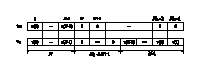
\includegraphics[keepaspectratio, scale=4]
					{parts/FourierAnalysis/imgs/FFT/arbitraryLengthFFT_to_powerOf2_FFT/u2,v2.eps}
					\caption{$u_2,v_2$の構造}
				\end{figure}
				このようにすると$u_2*v_2$の先頭$N$要素が$u*v$と一致する。
				\[ \text{FFT}(u_2*v_2) = \sqrt{N_2}\text{ FFT}(u_2) \text{ FFT}(v_2) \]
				より
				\[ \text{IFFT}(\sqrt{N_2}\text{ FFT}(u_2) \text{ FFT}(v_2)) \]
				により$u_2*v_2$を高速に計算し、結果の先頭$N$要素を切り出せば$u*v$を得る。
				得られた$u*v$の第$k$要素に$\frac{1}{\sqrt{N}} \exp \left(\pi i\frac{-k^2}{N}\right)$を掛ければ$x$のDFTが得られる。
				$v_2$のFFTや$\frac{1}{\sqrt{N}} \exp \left(\pi i\frac{-k^2}{N}\right) \;(k=0,1,\cdots,N-1)$は初回の計算結果を保存しておけば別の信号のDFTの計算で再利用できる。

	\part{Laplace変換}
    \chapter{複素指数関数入力に対する伝達関数の作用}
        \begin{shadebox}
            $A>0,\;\omega \in \realNumbers$とする。
            連続時間信号$f: \realNumbers \to \complexNumbers$を次のように定める。
            \[
                f(t) =
                \begin{cases}
                    A\NapierE^{i\omega t} & (t\geq 0) \\
                    0 & (t<0)
                \end{cases}
            \]
            $H: s\in\complexNumbers \mapsto H(s) \in \complexNumbers$をproperで既約な有理関数とする。
            また,$H$の極の実部は全て負であるとする。
            伝達関数が$H(s)$である連続時間システムに信号$f$を入力した時の出力を$g$とすると,十分大きい$t$に対して
            $g(t) \sim H(i\omega)f(t)$となる。
        \end{shadebox}
        \begin{proof}
            \quad\par
            $N_\text{p}$を$H(s)$の分母多項式の相異なる零点の個数とし,それら零点を$p_0,\dots,p_{N_\text{p}}$とする。
            零点$p_k$の次数を$N_{\text{p},k}$とし,$H(s)$の部分分数展開を
            \[ H(s) = c_0 + \sum_{k=1}^{N_\mathrm{p}} \sum_{l=1}^{N_{\mathrm{p},k}} \frac{c_{k,l}}{(s-p_k)^l} \]
            とする。
            ここに$c_0,c_{k,l}\;(k=1,\dots,N_\mathrm{p},l=1,\dots,N_{\mathrm{p},k})$は適当な複素数である。
            $f,g$のLaplace変換をそれぞれ$F,G$とすると$G(s) = H(s)F(s) = A H(s)/(s-i\omega)$である。
            これの部分分数展開に現れる,$1/(s-p_k)^l\;(k=1,\dots,N_\mathrm{p},l=1,\dots,N_{\mathrm{p},k})$に比例する項は逆Laplace変換すると$t^{l-1}\NapierE^{p_k t}$に比例する関数となり,$t\to\infty$で0に収束する。\hfill \rule{10cm}{0.4pt}(1)
            \par
            残りの項,すなわち$1/(s-i\omega)$に比例する項は$AH(i\omega)/(s-i\omega) = H(i\omega)F(s)$となる。
            以上より,十分大きい$t$に対して$g(t) \sim \ILPLC{H(i\omega)F(s)}(t) = H(i\omega)f(t)$となる。
        \end{proof}
        \section{系: 正弦波入力に対する伝達関数の作用}
            \begin{shadebox}
                $A>0,\;\omega \in \realNumbers$とする。
                連続時間信号$f_1,f_2: \realNumbers \to \realNumbers$を次のように定める。
                \[
                    f_1(t) =
                    \begin{cases}
                        A\cos\omega t & (t\geq 0) \\
                        0 & (t<0)
                    \end{cases}
                \]
                \[
                    f_2(t) =
                    \begin{cases}
                        A\sin\omega t & (t\geq 0) \\
                        0 & (t<0)
                    \end{cases}
                \]
                $H$を直前の定理と同じように定める。
                伝達関数が$H(s)$である連続時間\textcolor{red}{実}システムに信号$f_1,f_2$を入力した時の出力をそれぞれ$g_1,g_2$とすると,十分大きい$t$に対して
                \begin{align*}
                    g_1(t) &\sim |H(i\omega)|\cos(\omega t + \Arg\parens*{H(i\omega)}) \\
                    g_2(t) &\sim |H(i\omega)|\sin(\omega t + \Arg\parens*{H(i\omega)})
                \end{align*}
                となる。
            \end{shadebox}
            \begin{proof}
                \quad\par
                $f_1$について示す。
                $f_2$も同様に示せる。
                $f_1(t) = \Re{A\NapierE^{i\omega t}}$であり,実数システムだから出力は$A\NapierE^{i\omega t}$を入力したときの出力の実部と等しい。
                直前の定理の結果を用いて
                \[ g_1(t) = \Re{H(i\omega)A\NapierE^{i\omega t}} = \Re{|H(i\omega)|\NapierE^{i\Arg\parens*{H(i\omega)}}A\NapierE^{i\omega t}} = |H(i\omega)|\cos (\omega t + \Arg\parens*{H(i\omega)}) \]
            \end{proof}
            \begin{proof}
                (直接的な証明)
                \quad\par
                $f_1$について示す。
                $f_2$も同様に示せる。
                直前の定理の証明の(1)までは同じである。
                $f_1,g_1$のLaplace変換をそれぞれ$F_1,G_1$とすると
                \[ F_1(s) = \frac{As}{s^2+\omega^2} = \frac{A}{2}\left(\frac{1}{s+i\omega} + \frac{1}{s-i\omega}\right) \]
                であるから,$G_1(s) = H(s)F(s)$の部分分数展開のうち$1/(s+i\omega),\;1/(s-i\omega)$に比例する項を詳しく調べれば良い。
                $1/(s+i\omega)$の係数は
                \[ \left. G(s)X(s)(s+i\omega) \right|_{s\to-i\omega} = AG(-i\omega)/2\]
                となり,$1/(s-i\omega)$の係数は
                \[ \left. G(s)X(s)(s-i\omega) \right|_{s\to i\omega} = AG(i\omega)/2\]
                となる。
                よってこれらの項の和は
                \begin{align}
                    &\quad \frac{AG(-i\omega)/2}{s+i\omega} + \frac{AG(i\omega)/2}{s-i\omega} = \frac{A}{2}\left(\frac{G(-i\omega)}{s+i\omega} + \frac{G(i\omega)}{s-i\omega}\right) \nonumber\\
                    &= \frac{A}{2}\times\frac{1}{s^2+\omega^2}\left(G(-i\omega)(s-i\omega) + G(i\omega)(s+i\omega)\right) \nonumber\\
                    &= \frac{As}{s^2+\omega^2}\times\frac{1}{2}(G(i\omega)+G(-i\omega)) + \frac{A\omega}{s^2+\omega^2}\times\frac{-1}{2i}(G(i\omega)-G(-i\omega))
                \end{align}
                $G(s)$は有理式なので$G(-i\omega) = \conj{G(i\omega)}$となることに注意して
                \[ \frac{1}{2}(G(i\omega)+G(-i\omega)) = |G(i\omega)|\frac{1}{2}\left(\NapierE^{i\Arg\parens*{G(i\omega)}} + \NapierE^{-i\Arg\parens*{G(i\omega)}}\right) = |G(i\omega)|\cos\Arg\parens*{G(i\omega)} \]
                同様に
                \[ \frac{-1}{2i}(G(i\omega)-G(-i\omega)) = -|G(i\omega)|\sin\Arg\parens*{G(i\omega)} \]
                以上より,
                \begin{align*}
                    (1) &= |G(i\omega)|\left(\cos\Arg\parens*{G(i\omega)}\frac{As}{s^2+\omega^2} - \sin\Arg\parens*{G(i\omega)}\frac{A\omega}{s^2+\omega^2} \right) \\
                    g(t) &\sim \ILPLC{(1)}(t) = |G(i\omega)|\left(\cos\Arg\parens*{G(i\omega)}\cos\omega t - \sin\Arg\parens*{G(i\omega)}\sin\omega t \right) \\
                    &= |G(i\omega)|\cos\left(\omega t + \Arg\parens*{G(i\omega)}\right)
                \end{align*}
            \end{proof}
	\part{Z 変換}
	\chapter{基礎理論}
		\section{逆 Z 変換}
			\label{inv_Z_trans}
			\begin{shadebox}
				$X:\complexNumbers\to\complexNumbers$ は離散時間信号 $x:\integers\to\complexNumbers$ の Z 変換であるとする。
				このとき次式が成り立つ。
				\begin{equation}
					\label{eq:inv_Z_trans}
					x(n) = \frac{1}{2\pi i}\oint_C X(z)z^{n-1}\mathrm{d}z
				\end{equation}
				ここに積分路 $C$ は $X(z)$ のすべての極を含む反時計回りの単純閉曲線である。
			\end{shadebox}
			\begin{proof}
				\begin{align*}
					\frac{1}{2\pi i}\oint_C X(z)z^{n-1}\mathrm{d}z &= \frac{1}{2\pi i}\oint_C \parens*{\sum_{k=-\infty}^\infty x(k)z^{-k}}z^{n-1}\mathrm{d}z \\
					&= \sum_{k=-\infty}^\infty x(k)\frac{1}{2\pi i}\oint_C z^{n-k-1}\mathrm{d}z = \sum_{k=-\infty}^\infty x(k)\delta_{n,k} = x(n)
				\end{align*}
			\end{proof}
		\section{信号とその片側 Z 変換の一対一対応}
			離散時間信号 $x:\integers\to\complexNumbers$ とその片側 Z 変換 $X$ は非負の時間領域について一対一対応する。
			このことは \ref{inv_Z_trans} の証明から明らかである。
			片側 Z 変換の結果に対して式 \eqref{eq:inv_Z_trans} に於いて負の時刻を指定すると,結果は 0 である。
		\section{最終値定理}
			\begin{shadebox}
				$X(z)\;(z\in\complexNumbers)$を離散時間信号$x(n)\;(n \in \integers,\;\forall n<0,x(n)=0)$のZ変換とする。
				$\lim_{n\to\infty} x(n)$が存在するとき次が成り立つ。
				\[ \lim_{z\to1}(z-1)F(z) = \lim_{n\to\infty} x(n) \]
				但し上式に於ける$\lim_{z\to1}$では$z$が実軸上で右側から1に近づくことを意味する。
			\end{shadebox}
			\begin{proof}
				\quad\par
				$\alpha = \lim_{n\to\infty} x(n)$とする。
				発想としては,十分大きい$N\in\naturalNumbers$に対して$\sum_{k=N+1}^\infty x(k)z^{-k} \sim \sum_{k=N+1}^\infty \alpha z^{-k} = \alpha z^{-N}\frac{1}{z-1}$となることを利用する。
				\par
				任意の$\varepsilon \in (0,1)$に対してある$N\in\naturalNumbers$が存在して$\forall n\geq N,\;|x(n)-\alpha|<\varepsilon$となる。
				\begin{align*}
					\quad &\lim_{z\to1}(z-1)F(z) - \alpha = \lim_{z\to1}(z-1)z^N F(z) - \alpha \\
					&= \lim_{z\to1}(z-1)z^N\left(\sum_{k=0}^{N-1} x(k)z^{-k} + \sum_{k=N+1}^\infty x(k)z^{-k}\right) - (z-1)z^N\sum_{k=N+1}^\infty \alpha z^{-k} \\
					&= \lim_{z\to1}(z-1)z^N \sum_{k=N+1}^\infty (x(n) - \alpha)z^{-k} \quad \left(\sum_{k=0}^{N-1}\text{の項は極限で消える}\right) \tag{1} \\
					|(1)| &\leq \lim_{z\to1}(z-1)z^N \sum_{k=N+1}^\infty |x(n) - \alpha|z^{-k} < \lim_{z\to1}(z-1)z^N \sum_{k=N+1}^\infty \varepsilon z^{-k} = \varepsilon
				\end{align*}
			\end{proof}
		\section{複素指数関数入力に対する伝達関数の作用}
			\begin{shadebox}
				$A>0,\;\omega \in \realNumbers$とする。
				離散時間信号$x: \realNumbers \to \complexNumbers$を次のように定める。
				\[
					x(n) =
					\begin{cases}
						Ae^{i\Omega n} & (n\geq 0) \\
						0 & (n<0)
					\end{cases}
				\]
				$H: z\in\complexNumbers \mapsto H(z) \in \complexNumbers$を,$1/z$を変数とした有理式として既約であるような有理関数とする。
				また,$H$の極の絶対値は全て1未満であるとする。
				伝達関数が$H(z)$である離散時間システムに信号$x$を入力した時の出力を$y$とすると,十分大きい$n$に対して
				$y(n) \sim H(\NapierE^{i\Omega})x(n)$となる。
			\end{shadebox}
			\begin{proof}
				\quad\par
				$N_\text{p}$を$H(s)$の相異なる極の個数とし,それら極を$p_0,\dots,p_{N_\text{p}}$とする。
				極$p_k$の次数を$N_{\text{p},k}$とし,$H(z)$の部分分数展開を
				\[ H(z) = c_0 + \sum_{k=1}^{N_\mathrm{p}} \sum_{l=1}^{N_{\mathrm{p},k}} \frac{c_{k,l}}{(1-p_kz^{-1})^l} \]
				とする。
				ここに$c_0,c_{k,l}\;(k=1,\dots,N_\mathrm{p},l=1,\dots,N_{\mathrm{p},k})$は適当な複素数である。
				$x,y$のZ変換をそれぞれ$X,Y$とすると$Y(z) = H(z)F(z) = A H(z)/(1-\NapierE^{i\Omega}z^{-1})$である。
				これの部分分数展開に現れる,$1/(1-p_k z^{-1})^l\;(k=1,\dots,N_\mathrm{p},l=1,\dots,N_{\mathrm{p},k})$に比例する項は逆Z変換すると$n$の多項式と公比$p_k$の等比級数の積となり,$n\to\infty$で0に収束する。
				(このことはZ変換の性質: 時間シフト$\mathcal{Z}[x(n+k)] = z^kX(z)$,およびZ領域微分$\mathcal{Z}[nx(n)] = -z\derivLong{\mathcal{Z}[x(n)]}{z}{}$を繰り返し用いることで分かる)
				\par
				残りの項,すなわち$1/(1-\NapierE^{i\Omega}z^{-1})$に比例する項は$AH(\NapierE^{i\Omega})/(1-\NapierE^{i\Omega}z^{-1}) = H(\NapierE^{i\Omega})X(z)$となる。
			\end{proof}
	% \chapter{IIRフィルタの計算手順}
	% 	\begin{figure}[H]
	% 		\centering
	% 		\includegraphics[keepaspectratio, scale=5]
	% 		{\currfiledir/figs/IIR-filter/calculationMethod/blockDiagram.pdf}
	% 		\caption{IIRフィルタのブロック図の例}
	% 	\end{figure}
	% 	上の例で示したIIRフィルタの出力は以下の手続きで計算できる(仕事で関わっていたデジタル無線機の信号処理部でそうやっていた)。
	% 	\begin{enumerate}
	% 		\item $D_1,\cdots D_4 \leftarrow 0$
	% 		\item $n \leftarrow 0$
	% 		\item $\alpha \leftarrow a_1D_1 + \cdots a_4D_4$
	% 		\item $\beta \leftarrow b_1D_1 + \cdots b_4D_4$
	% 		\item $\gamma \leftarrow x(n) + \beta$
	% 		\item $y(n) \leftarrow \alpha + a_0\gamma$
	% 		\item $D_4 \leftarrow D_3,\;D_3 \leftarrow D_2,\;D_2 \leftarrow D_1,\;D_1 \leftarrow \gamma$
	% 		\item $n \leftarrow n+1$
	% 		\item $n$が$x$の定義域の末尾に達しているなら終了。そうでないなら3に戻る。
	% 	\end{enumerate}
	\part{応用}
    \chapter{NCO}
    \section{位相の下位ビット切り捨てとスプリアス}
        数値制御発振器(Numerical Controlled Oscillator; NCO) の Look-up table (LUT) のサイズを減らすために位相の下位ビットを切り捨てて出力した場合、(離散時間信号として)スプリアスを生じる。
        ここでは簡単のため、周波数が最小(1クロックでの位相の増加が1)の正弦波について考える。
        \subsection{主張}
            \begin{shadebox}
                $N,W\in\naturalNumbers,\;N>W$とする。
                位相加算器の語長が $N$ であり、1クロックあたりの位相の増加は1であるとする。
                位相の下位 $W$ ビットを切り捨てた場合、DFT に於いて周波数が $1 + 2^{N-W}m\;(m\in\integers,\;0<m\geq 2^{W-1})$ のスプリアスが生じる。
            \end{shadebox}
        \subsection{導出}
            \begin{proof}
                \quad\par
                NCO の出力は次式である。
                \[ x_W(n) = \exp\parens*{i\frac{2^W\floor{n/2^W}}{2^N}2\pi} \]
                これの DFT は次式である。
                \begin{align*}
                    X_W(k) &= \frac{1}{\sqrt{2^N}} \sum_{n=0}^{2^N-1} x_W(n)\exp\parens*{-ik\frac{n}{2^N}2\pi} \\
                    &= \frac{1}{\sqrt{2^N}} \sum_{m=0}^{2^{N-W}-1} \exp\parens*{i\frac{2^W m}{2^N}2\pi} \sum_{l=0}^{2^W-1} \exp\parens*{-ik\frac{2^W m + l}{2^N}2\pi} \\
                    &= \frac{1}{\sqrt{2^N}} \sum_{l=0}^{2^W-1} \exp\parens*{-ik\frac{l}{2^N}2\pi} \sum_{m=0}^{2^{N-W}-1} \exp\parens*{-i(k-1)\frac{m}{2^{N-W}}2\pi} \\
                    &= \frac{1}{\sqrt{2^N}} \frac{1-\exp\parens*{-ik\frac{2^W}{2^N}2\pi}}{1-\exp\parens*{-ik\frac{2\pi}{2^N}}}\frac{1-\exp\parens*{-i(k-1)2\pi}}{1-\exp\parens*{-i(k-1)\frac{2\pi}{2^{N-W}}}} \\
                    &= \frac{1}{\sqrt{2^N}}\frac{\exp\parens*{-ik\frac{2^W}{2^N}\pi}}{\exp\parens*{-ik\frac{\pi}{2^N}}}\frac{\exp\parens*{ik\frac{2^W}{2^N}\pi} - \exp\parens*{-ik\frac{2^W}{2^N}\pi}}{\exp\parens*{ik\frac{\pi}{2^N}} - \exp\parens*{-ik\frac{\pi}{2^N}}}\frac{\exp\parens*{-i(k-1)\pi}}{\exp\parens*{-i(k-1)\frac{\pi}{2^{N-W}}}} \\
                    &\phantom{=}\times\frac{\exp\parens*{i(k-1)\pi} - \exp\parens*{-i(k-1)\pi}}{\exp\parens*{i(k-1)\frac{\pi}{2^{N-W}}} - \exp\parens*{-i(k-1)\frac{\pi}{2^{N-W}}}} \\
                    &= \frac{1}{\sqrt{2^N}} \exp\parens*{ik\frac{1-2^W}{2^N}\pi}\frac{\sin\parens*{\frac{k}{2^{N-W}}\pi}}{\sin\parens*{\frac{k}{2^N}\pi}}\exp\parens*{i(k-1)\parens*{\frac{1}{2^{N-W}}-1}\pi}\frac{\sin\parens*{(k-1)\pi}}{\sin\parens*{\frac{k-1}{2^{N-W}}\pi}} %\\
                    %&= \sqrt{2^N} \exp\parens*{ik\frac{1-2^W}{2^N}\pi}\frac{\sinc\parens*{\frac{k}{2^{N-W}}\pi}}{\sinc\parens*{\frac{k}{2^N}\pi}}\exp\parens*{i(k-1)\parens*{\frac{1}{2^{N-W}}-1}\pi}\frac{\sinc\parens*{(k-1)\pi}}{\sinc\parens*{\frac{k-1}{2^{N-W}}\pi}}
                \end{align*}
                但し、上式に於いて $\sin/\sin$ の部分で $0/0$ の不定形が生じるような $k$ の値 $k'$ に対しては、値域を一時的に実数に広げて $k\to k'$ の極限を取る。
                このようにしても等式が成り立つことは、$k'$ に対して $\Sigma$ を直接計算することで容易に確かめられる。
                \par
                $\sin\parens*{(k-1)\pi}/\sin\parens*{\frac{k-1}{2^{N-W}}\pi}$ は $k$ に関する $2^{N-W}$ 周期関数であり、$k = 1 + 2^{N-W}m\;(m\in\integers,\;0<m\geq 2^{W-1}$ のときに $2^{N-W}$ となり、それ以外では 0 である。
            \end{proof}
        \subsection{数値例}
            次の図は $N=8,\;W=0,2$ の例である。
            \begin{figure}[H]
                \centering
                \includegraphics[keepaspectratio, scale=0.7]
                {\currfiledir/figs/real-part_of_NCO_output.pdf}
                \caption{NCO の出力の実部}
            \end{figure}
            \begin{figure}[H]
                \centering
                \includegraphics[keepaspectratio, scale=0.7]
                {\currfiledir/figs/Log10[Abs[DFT]].pdf}
                \caption{$\log_{10}X_W$}
            \end{figure}
    \chapter{Nyquist ISI 基準}
    これは大雑把に言うと Fourier 変換が存在する連続時間信号 $h:\realNumbers\to\complexNumbers$ が 1 つの例外の時刻を除いて、ある周期 $\Ts>0$ (s は symbol の意味)の整数倍の時刻で 0 になるための必要十分条件である。
    限定された周波数帯域を使って通信する際に受信側で情報を正しく復元するために重要な性質であり、詳細は \cite{Nyquist_ISI_crit} にある。
    数式で表すと次である。
    \[
        h(n\Ts) = \begin{cases}
            1 & n=0 \\
            0 & n\in\integers\setminus\{0\}
        \end{cases}
        \iff \forall f\in\realNumbers,\;\frac{1}{\Ts}\sum_{n=-\infty}^\infty H(f-n/\Ts) = 1
    \]
    ここに $H$ は $h$ の Fourier 変換である。
    \cite{Nyquist_ISI_crit} には $\Rightarrow$ の証明のみがある。
    本書では $\Leftarrow$ を証明する。
    \begin{proof}
        \begin{align*}
            1 &= \frac{1}{\Ts}\sum_{n=-\infty}^\infty H(f-n/\Ts) = \frac{1}{\Ts}\sum_{n=-\infty}^\infty\integrate{-\infty}{\infty}{h(t)\exp\parens*{-i2\pi(f-n/\Ts)t}}{}{t} \\
            &= \frac{1}{\Ts}\integrate{-\infty}{\infty}{h(t)\exp(-i2\pi ft)\sum_{n=-\infty}^\infty\exp\parens*{i2\pi nt/\Ts}}{}{t} \tag{1}
        \end{align*}
        ここで次の関係式を使う(Dirac のデルタ関数の無限和に関する頻出の関係式であり、類似の形の式が以前の部や章で使われている)。
        \[ \sum_{n=-\infty}^\infty\exp\parens*{i2\pi nt/\Ts} = 2\pi\Ts\sum_{n=-\infty}^\infty\delta(2\pi t-2\pi\Ts n) = \Ts\sum_{n=-\infty}^\infty\delta(t-n\Ts) \]
        これを式 (1) に適用して次式を得る。
        \begin{align*}
            1 &= \integrate{-\infty}{\infty}{h(t)\exp\parens*{-i2\pi ft}\sum_{n=-\infty}^\infty\delta(t-n\Ts)}{}{t} = \sum_{n=-\infty}^\infty\integrate{-\infty}{\infty}{h(t)\exp\parens*{-i2\pi ft}\delta(t-n\Ts)}{}{t} \\
            &= \sum_{n=-\infty}^\infty h(n\Ts)\exp\parens*{-i2\pi fn\Ts}
        \end{align*}
        右辺は $f$ に関する周期 $1/\Ts$ の関数の Fourier 級数であり、$h(n\Ts)$ は Fourier 係数である。
        左辺が 1 であることから $h(0) = 1,\;h(n\Ts)\;(n\neq 0) = 0$ である(より丁寧に論じるなら、前記の式の両辺に $\exp(i2\pi fk\Ts)\;(k\in\integers)$ を掛けて区間 $[-1/(2\Ts),1/(2\Ts)]$ で積分する。その結果が $k$ にどう依存するかを調べる)。
    \end{proof}
    \chapter{信号検出}
    \section{位置特定に於けるcos類似度による方法と最良近似による方法の等価性}
        複素数列で表される受信信号$\{s_i\}$の中から特定のパターン(「参照信号」と呼ぶ)を見つけ出したい時がある。
        例えば無線通信に於いては送信機から「同期ワード (Sync Word, SW)」と呼ばれる数十bit分の変調信号が一定周期で送出されており、これが「フレーム」と呼ばれる単位の区切り位置の決定に使われる。
        受信機は常にSWを探索し、フレームの区切り位置を絶えずトラッキングする必要がある。
        なぜならば、送信機,受信機に搭載されているクロック発生器には僅かだが誤差があり、受信機から見た送信機の送出する信号の時間軸は少しずつズレていくからである。
        \par
        今、受信信号列の全体的な位相には関心が無いものとする。
        つまり、信号全体に大きさ1の複素定数を乗算する操作は受信側の信号処理にとって影響がないものとする。
        現実の無線機で言えば、例えば$\pi/4$シフトQPSKがそうである。
        \par
        受信信号から参照信号を検出する方法として、直観的に次の2つの方法を思いつくだろう。
        \subsection{手法1: cos類似度の絶対値の最大化}
            \label{手法1: cos類似度の絶対値の最大化}
            参照信号の長さを$L\in\naturalNumbers$, 参照信号を$\bm{d} \in \complexNumbers^L$, 受信信号中のテスト領域を$\bm{s}^{(i)} \coloneqq [s_i,s_{i+1},\dots,s_{i+L-1}]^\top \in \complexNumbers^L$とするとき、$\bm{d}$と$\bm{s}^{(i)}$の$\cos$類似度の複素数版
            \[ \frac{\bm{d}^*\bm{s}^{(i)}}{\norm{\bm{d}}_2\norm{\bm{s}^{(i)}}_2} \]
            の位相を無視し、絶対値の2乗(2乗を使うのは、平方根の計算を無くして計算量を抑える為)で評価する。
            $\norm{\bm{d}}_2$は$\bm{s}^{(i)}$に依存しないので評価値同士の大小比較に必要ないから取り除く。
            すると評価関数$c$として次式を得る。
            \[ c(i) = \frac{|\bm{d}^*\bm{s}^{(i)}|^2}{\norm{\bm{s}^{(i)}}_2^2} \]
            これが最大となる$i$を参照信号の存在位置と見做す。
        \subsection{手法2: 最良近似}
            \ref{手法1: cos類似度の絶対値の最大化}で定義した記号をここでも用いる。
            受信信号中の参照信号は「参照信号+ゲイン変化+位相回転+ノイズ」の形で存在している。
            そこで、参照信号に定数$\alpha$を掛けて$\bm{s}^{(i)}$との差を取った絶対値の2乗を参照信号のL-2ノルムの2乗で正規化した値が最小となるように$\alpha$を選び、そのときの差の絶対値の2乗が最小になるような位置をもって参照信号の存在位置と見做す。
            評価関数$\tilde{c}$は次式である。
            \[ \tilde{c}(i) = \frac{1}{\norm{\bm{s}^{(i)}}_2^2}\min_{\alpha \in \complexNumbers}\norm{\alpha\bm{d} - \bm{s}^{(i)}}_2^2 \]
            正規化する理由は、テスト領域の強度の影響を減らすためである。
            テスト領域の形が参照信号と大きく異なっていても、テスト領域の強度が小さければ$\min_{\alpha \in \complexNumbers}\norm{\alpha\bm{d} - \bm{s}^{(i)}}_2^2$は小さくなり、誤った推定結果を導き得る。
            上の最小化問題の解は解析的に求められる。
            $f(\alpha) \coloneqq \norm{\alpha\bm{d} - \bm{s}^{(i)}}_2^2$について微小な$\Delta\alpha$を考え、$f(\alpha+\Delta\alpha) - f(\alpha)$の変化量の$\Delta\alpha$の1次の項が0になるような$\mathring{\alpha}$が解である。これは次式である。
            \[
                \mathring{\alpha} = \frac{\bm{d}^*\bm{s}^{(i)}}{\norm{\bm{d}}_2^2}
            \]
            よって$\tilde{c}(i)$は次式である。
            \[ \tilde{c}(i) = \frac{1}{\norm{\bm{s}^{(i)}}_2^2}\norm{\bm{s}^{(i)} - \frac{\bm{d}^*\bm{s}^{(i)}}{\norm{\bm{d}}_2^2}\bm{d}}_2^2 \]
        \subsection{手法1,2の等価性}
            実は手法1と2は等価である。
            すなわち次の命題は真である。
            \[ \frac{1}{\norm{\bm{s}^{(i)}}_2^2}\norm{\bm{s}^{(i)} - \frac{\bm{d}^*\bm{s}^{(i)}}{\norm{\bm{d}}_2^2}\bm{d}}_2^2 < \frac{1}{\norm{\bm{s}^{(j)}}_2^2}\norm{\bm{s}^{(j)} - \frac{\bm{d}^*\bm{s}^{(j)}}{\norm{\bm{d}}_2^2}\bm{d}}_2^2 \iff \frac{|\bm{d}^*\bm{s}^{(i)}|^2}{\norm{\bm{s}^{(i)}}_2^2} > \frac{|\bm{d}^*\bm{s}^{(j)}|^2}{\norm{\bm{s}^{(j)}}_2^2} \]
            これを示す。
            \begin{align*}
                \frac{1}{\norm{\bm{s}^{(i)}}_2^2}\norm{\bm{s}^{(i)} - \frac{\bm{d}^*\bm{s}^{(i)}}{\norm{\bm{d}}_2^2}\bm{d}}_2^2 &= \frac{1}{\norm{\bm{s}^{(i)}}_2^2}\left[ \norm{\bm{s}^{(i)}}_2^2 + \frac{|\bm{d}^*\bm{s}^{(i)}|^2}{\norm{\bm{d}}_2^4}\norm{\bm{d}}_2^2 - \frac{\bm{d}^*\bm{s}^{(i)}}{\norm{\bm{d}}_2^2}{\bm{s}^{(i)}}^*\bm{d} - \frac{\conj{\bm{d}^*\bm{s}^{(i)}}}{\norm{\bm{d}}_2^2}\bm{d}^*\bm{s}^{(i)} \right] \\
                &= \frac{1}{\norm{\bm{s}^{(i)}}_2^2}\left[ \norm{\bm{s}^{(i)}}_2^2 + \frac{|\bm{d}^*\bm{s}^{(i)}|^2}{\norm{\bm{d}}_2^2} - 2\frac{|\bm{d}^*\bm{s}^{(i)}|^2}{\norm{\bm{d}}_2^2} \right] \\
                &= 1 - \frac{|\bm{d}^*\bm{s}^{(i)}|^2}{\norm{\bm{d}}_2^2}
            \end{align*}
            であり、
            \[ 1 - \frac{|\bm{d}^*\bm{s}^{(i)}|^2}{\norm{\bm{d}}_2^2} < 1 - \frac{|\bm{d}^*\bm{s}^{(j)}|^2}{\norm{\bm{d}}_2^2} \iff \frac{|\bm{d}^*\bm{s}^{(i)}|^2}{\norm{\bm{s}^{(i)}}_2^2} > \frac{|\bm{d}^*\bm{s}^{(j)}|^2}{\norm{\bm{s}^{(j)}}_2^2} \]
            であることから命題が真であることがわかる。


	\begin{thebibliography}{99}
	\end{thebibliography}
\end{document}
